

\chapter{Boxes and glue in TeX}

\setlength{\columnsep}{2em}
{\it Once you understand TEX's concept of glue, you may well decide that
it was misnamed; real glue doesn't stretch or shrink in such ways, nor does it
contribute much space between boxes that it welds together. Another word like
\emph{spring} would be much closer to the essential idea, since springs have a natural
width, and since different springs compress and expand at different rates
under tension. But whenever the author has suggested changing \tex's terminology,
numerous people have said that they like the word \emph{glue} in spite of its
inappropriateness; so the original name has stuck. }
\smallskip

{\hfill  ---  Donald E. Knuth}

\medskip   %smallskip 



\parindent1em




\newthought{Traditional typesetting} was a task that depended on assembling the types and inserting them one by one on holding frames. In a way it was an assembly of boxes.
The \tex typesetting system uses a similar model of boxes to typeset content but in addition it also uses the concept of glue to stretch or shrink the text so that it will look better typographically. Boxes contain
typeset objects, such as text, mathematical displays, and pictures, and glue
is flexible space that can stretch and/or shrink by amounts that are under
user control.

\topline

Some example is placed her\\
and

\bottomline

\section*{Boxes}

Boxes in \tex have  a rectangular shape but have
three associated measurements called \emph{height}, \emph{width}, and \emph{depth}.
Figure \ref{fig:boxes} shows a 
picture of a typical box, showing its so-called \emph{reference point} and \emph{baseline}

The reason that they have three dimensions is that a character of text has normally three dimensions as shown in figure \ref{fig:boxes}. As characters need to be lined on a baseline, the depth provides a datum point on which they can be aligned and the depth provides a measure of the portion of the character that is below the baseline.


Boxes and glue are the main tools of \tex. The box can hold text and other items. Glue is simply spacing. It can be horizontal or veritcal spacing, and it can be made as rigid or as flexible as desired.



\begin{minipage}{\linewidth}
\textbf{One important feature of \tex is that it has no knowledge of the shape of the characters it typesets, just the dimensions of each character box.}
\end{minipage}
\medskip

When \tex is typesetting, it is normally in horizontal mode, such as while
it is working on this paragraph. Otherwise, \tex can be in vertical mode, or
in math mode, or three others described in Chapter 13 of The \texbook.
Two low-level TEX commands for boxes are \cmd{hbox}, for a horizontal box,
and \cmd{vbox} for a box in vertical mode. In the latter, \tex is normally still
collecting material for display from right to left: it is not building up a
column of text, as in classical Chinese writing.

In both kinds of boxes, the result is an unbreakable object that acts
much like a single character. \tex reads input as a string of characters,
then breaks that string up in words, each of which forms a box. 
\emph{Word boxes}\index{word boxes}
are then collected into lines, lines into paragraphs, and paragraphs into a
page galley. The space between the words can be normal \emph{interword space},
or \emph{sentence-ending} space, which is somewhat larger in English-language
typesetting, and the space is normally glue, rather than of fixed size.

\tex has a sophisticated mathematical algorithm for figuring out the
best way to stretch or shrink interbox glue to optimize the appearance of
lines and paragraphs. Every so often, \tex checks to see whether it has
enough material saved on the growing page galley to fill a complete output
page, and it asynchronously (and effectively, unpredictably) calls the
output routine whose job it is to figure out where the page break should
happen, ship out a completed page to the |DVI|  file, and replace the galley by
whatever is left over.

In traditional \tex you  can force a line break with the carriage-return command \cmd{cr},
and a page break with the command \cmd{eject}, but \tex is an expert system,
and normally handles line and page breaking on its own. \latex provides its own commands such as \cmd{clearpage} and \cmd{newpage} and so do all other \tex based systems.

\latex does not modify any of \tex's algorithms but simply it is a set of implemenation
macros.

\section{Units of measurement in TEX}

\tex allows you to specify sizes of typographical objects in any of nine different
units:


\begin{table}[htbp]
\begin{center}
\begin{tabular}{llp{5cm}}
\toprule
bp &big point &1 inch is exactly 72 bp; the PostScript pagedescription language uses these units, but just calls them points\\
cc &cicero: &1 cc is exactly 12 didot points, and is thus the European  analogue of the pica\\
cm &centimeter: &1 in is exactly 2.54 cm\\
dd &didot point: &1 dd is (1238/1157) pt, and is a typographical unit common in some parts of Europe\\
in &inch: &an archaic unit, roughly the width of a man's thumb; it has been discarded by most countries, but still used in the USA and its sattelites.\\
mm &millimeter: &1 in is exactly 25.4 mm\\
pc &pica: &1 pc is exactly 12 pt\\
pt &printer's point: &1 in is exactly 72.27 pt\\ 
sp &scaled point: &1 pt is exactly $2^{16}$ = 65536 sp.\\
\bottomrule
%\caption{TeX units of measure}
\end{tabular}
\end{center}
\end{table}



The units can be separated from their numeric value with optional space, so
\texttt{3pc} and \verb*+3 pc+ are equivalent. The little half box in the latter is a convenient
way to indicate explicit spaces in typewriter text. It can be printed by typing \cmd{char32}.

Internally, \tex\ stores dimensions as integral numbers of scaled points:
1 sp is tiny ---  smaller than the wavelength of visible light.\footnote{The visible light has wavelengths from 380--450 nm for violet up to 620--750 nm for red (sp = 280 nm} It is sometimes
useful to create objects that small so that they differ from empty objects,
but are nevertheless invisible. It also ensures that TeX will look the same irrespective on which computer you actually compiled your document.

\tex deals only with 32-bit integer words, and does not take advantage
of extra precision available on historical machines with larger words. The
lower 16 bits of a dimension can be viewed as a fractional number of points,
and the uppermost bit is needed for a sign (0 for plus, 1 for minus). That
leaves 15 bits to hold an integral number of points, but TEX only expects 14
to be used, so that addition of two dimensions does not overflow. Thus, the
largest dimension in TEX is exactly 214 + (1 26) points, or about 5.758  
meters or 18.89 feet.

\tex has several kinds of special storage locations, called registers, numbered
from 0 to 255. For example,\cs{dimen0} can hold a fixed dimension,
which can be specified in any of the nine units of measurement that are
recognized by \tex.

Here is how you can assign a dimension to a register, and then have \tex
display it back for you:

\begin{teXXX}
\dimen1 = 25.4mm (*@\protect\footnote{You shouldn't assign dimenensions to primitive registers, but rather use one of the allocation schemes provided by LaTeX to do so.}  @*)
\the\dimen1
\end{teXXX}

This will result in
\dimen1 = 25.4mm

\the\dimen1


Notice that \tex’s output is always in points, showing that it converts different
input units to a common system of measurement.

You can convert a dimension to the much-smaller units of scaled points
by assigning it to another kind of \tex register designed to hold signed integers,
the\cs{count0} through\cs{count255} registers:

\begin{texexample}{}{}
\dimen4 = 1pt
\count4 = \dimen4
\the\count4
\end{texexample}

{\noindent This time we get the size as \texttt{sp} as 65536 }


You might have noticed that the conversion from inches to points was not
quite what we claimed in the summary of \tex units. Here is how to see the
differences:

\verb+\dimen1 = 1in+


\section{Skip registers}
\index{registers!skip}
\begin{macro}{\skip}
\tex glue is specified as a fixed dimension, and optionally, with a plus and/
or minus dimension. Along with \cs{dimen} registers, TEX has glue registers,
called \cs{skip0} through \cs{skip255}. Here is how you can save glue settings in
 registers, and ask \tex to display the contents of one of them:
\end{macro}

\begin{teXXX}
  \skip1 = 10pt
  \skip2 = 10pt plus 3pt
  \skip3 = 10pt minus 2pt
  \skip4 = 10dd plus 3dd minus 2dd
  \showthe \skip4
  > 10.70007pt plus 3.21002pt minus 2.14001pt.
\end{teXXX}


The four sample glue settings store, respectively, \textit{fixed glue}, \textit{stretchable
glue}, \textit{shrinkable glue}, and \textit{flexible glue} that can both stretch and shrink,
but only up to a specified amount. Interword and intersentence spaces are
generally defined with glue like this, so that if more stretch or shrink of
\index{glue}\index{glue!flexibe}\index{glue!stretchable}\index{glue!shrinkable}

\begin{teX}
\dimen2 = 72.27pt
\count1 = \dimen1
\count2 = \dimen2
\showthe \count1
> 4736286.
\showthe \count2
> 4736287.
\end{teX}

The two values differ by the tiny value 1 \textit{sp}, so we can in practice ignore
that difference. If we use higher-precision arithmetic, we find the exact
decimal equivalents of the fractions as

\begin{teX}
4 736 286=65 536 = 72.269 989 013 671 875;
4 736 287=65 536 = 72.270 004 272 460 937 5;
4 736 286.72=65 536 = 72.27
\end{teX}


Actually \tex uses that last relation as the definition of the conversion of
inches to scaled points, so that our assignment of 1 in to \verb+\dimen1+ has to
be rounded to the nearest integral number of scaled points. That is why
in the round-trip conversion from decimal to binary and back to decimal,
1 in became 72.26999 pt. \tex guarantees that its output decimal numbers
are always converted on input back to the original binary numbers from
whence they came. For more on the story of \tex’s I/O conversions, see [3].


Both \tex and \latex define a number of predefined dimensions and these are discussed in the relevant Chapters discussing the \latex kernel. For example you might have come across the \cs{jot}, which is defined by \latex as:

\begin{teXX}
\newdimen\jot
This is some sample text with a one |\jot| left indentation. Which is really too small to see in a paragraph.
\jot=3pt
\end{teXX}

Defining |\parindent=jot| we can see that the indentation almost disappeared. This is obvious since |\jot| is used normally for maths.

Glue is the binder that lets \tex\ do its job. This chapter discusses some
preset forms of glue and their uses. Along with glue parameters there are a
number of special commands for inserting glue. The most interesting have
different degrees of infinity, namely |\hfil|, |\hfill|, |\hfilneg|, |\hss|,
and their vertical counterparts. 

Because of the special spacing requirements of mathematics, \tex\ defines
skips and spacing that are valid in mathematics mode only. Examples are the
are the special preset |mu| glues of |\thickmuskip|,
|\medmuskip|, |\thinmuskip|.
The |\newskip| and |\newmuskip| commands allocate skip (or really glue)
or muskip registers respectively for special uses. For example the specific
glues surrounding section heads are held in glue registers. 

It should be noted that the various |\...muskip| do not cause horizontal
spacing in math mode by themselves. They are used with |\mskip| to actually
cause the insertion of the glue.

These are all various forms of horizontal (or math) mode commands that insert
infinite quantities of glue. |\hfil|, |\hfill|, |\hfilneg|, and |\hss| insert
|plus 1fil|, |plus 1fill|, |minus 1fil|, and |plus 1fil minus 1fil|. 
The first two are {\it stretch} glues, the third is {\it shrink} glue and the
last is both. It
should be noted that when \tex\ tries to stretch or shrink glue values, they
vary according to their value. If there exists both |fil| and finite value
glue in a box or line, then all the stretch if it is |plus| glue 
or shrink if it is |minus| glue will be in
the section with the |fil| glue. If there is |fill| glue and either |fil| or
finite glue, then all the stretch or shrink will be in the |fill| sections.
Similarly with |filll| glue, which is not supplied in as readily usable form.
The difference in behaviour between |\hfil| and |\hss| is that |\hss| glue
will allow the contents of a box to spill outside without resulting in an
overfull box while |\hfil| will only fill or push contents to the edge of the
box. The major use for these glues are to center or to force stuff to either
edge of a box.  For instance this

\begin{texexample}{}{}
\def\aline{\vrule \hfil one \hfil two \hfil three 
         \hfill four \hfil five \hfil six 
         \hfill seven \hfil eight \hfil nine\vrule}

\aline

This is a preset |mu| glue. |\medmuskip = 4mu plus 2mu minus 4mu| for use
with |\mskip|. This is \hbox{\strut\vrule$\mskip\medmuskip$\vrule}.
\end{texexample}


\begin{macro}{\newskip}
The command \cs{newskip}\meta{skip name} assigns a new skip or glue register to
the name |\<skip name>|. Glue values may be assigned to it by |\<skip name> [=] <glue>|.
This assigns a new muskip or muglue register to the name |\<muskip name>|. Glue
values may be assigned to it by |\<muskip name> [=] <muglue>|.

This is a preset |mu| glue. |\thickmuskip = 5mu plus 5mu| for use
with |\mskip|. This is \hbox{\strut\vrule$\mskip\thickmuskip$\vrule}.

This is a preset |mu| glue. |\thinmuskip = 3mu| for use
with |\mskip|. This is \hbox{\strut\vrule$\mskip\thinmuskip$\vrule}
\end{macro}


\newskip\hides 
\hides= -1000pt% plus 1fill

atest atest

\hskip\hides atest

\hides= -1000pt  plus 1fill

atest atest

\hskip\hides atest

|\vfil \vfill|

|\vfilneg|

|\vss|

These are the vertical analogues to the infinite horizontal glues and act in
much the same manner. See the section on |\hfil ...|.
 



\normalsize



\section{Glue}

\tex joins the boxes it creates with some special mortar as Knuth writes, called glue. To understand how glue works we will
borrow a figure from the \tex Book.

\begin{figure}
 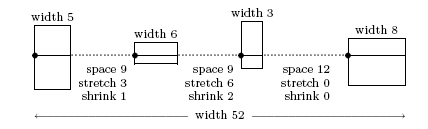
\includegraphics[width=0.9\linewidth]{glue}
  \caption{Glue in \TeX}
  \label{fig:glue}
\end{figure}


\section{How to specify glue}

The usual way to specify \textit{glue} to \tex is
$<dimen>< plus~dimen><minus~dimen>$

where the plus and minus are optional and assumed to be zero if not
present; plus\index{glue!plus} introduces the amount of stretchability\index{glue!stretchability}, minus introduces the amount of shrinkability \index{glue!shrinkability}. 

For example, Appendix B of the TexBook defines \cs{medskip} to be an abbreviation for
|\vskip6pt plus2pt minus2p|. The normal-space component of glue must always be
given as an explicit dimen, even when it is zero. The ability of \TeX to stretch and shrink this glue has given it its beautiful looks. Strangely enough, although the algorithm is public it has not been used widely in other software.



\subsection*{hfil and hfill}

{\obeylines
{This text will be flush left.\hfil}
{\hfil This text will be flush right.}
{\hfil This text will be centered.\hfil}
{Some text flush left\hfil and some flush right.}
{Alpha\hfil centered between Alpha and Omega\hfil Omega}
{Five\hfil words\hfil equally\hfil spaced\hfil out.}
}

Consider the following definitions:

\begin{verbatim}
\def\centerlinea#1{\hfil#1\hfill}
\def\centerlineb#1{\hfill#1\hfill}
\def\centerlinec#1{\hss#1\hss}
We define quickly a \cs{lineX}\footnote{Strange but my \LaTeX\ distribution has not got on. (This definition is from \texttt{plain.sty}}

\def\lineX{\hbox to\hsize}
\def\lineX{\hbox to\hsize}
\def\centerlinea#1{\hfil#1\hfil}
\def\centerlineb#1{\hfill#1\hfill}
\def\centerlinec#1{\hss#1\hss}

\lineX{\centerlinea{\test}}
\lineX{\centerlineb{\test}}
\lineX{\centerlinec{\test}}
\centerline{\test}
\begin{center}\test\end{center}

\end{verbatim}


\section{Specifying glue amounts}

\tex glue is specified as a fixed dimension, and optionally, with a plus and
or minus dimension. Along with \cs{dimen} registers, TEX has glue registers,
called \cs{skip0} through \cs{skip255}. Here is how you can save glue settings in
\tex registers, and ask \tex to display the contents of one of them:

\begin{teX}
\skip1 = 10pt
\skip2 = 10pt plus 3pt
\skip3 = 10pt minus 2pt
\skip4 = 10dd plus 3dd minus 2dd
\the \skip4
\end{teX}


\texttt{> 10.70007pt plus 3.21002pt minus 2.14001pt}

The four sample glue settings store, respectively, {\em fixed glue}, {\em  stretchable
glue}, {\em shrinkable glue}, and {\em flexible glue}  that can both stretch and shrink,
but only up to a specified amount. Interword and intersentence spaces are
generally defined with glue like this, so that if more stretch or shrink of  a
re underfull (too little text to fill the line), or overfull (too much text in the
line).



\section{Overfull lines}

Although overfull lines are reported in the \tex log file, they can be hard
to find in the typeset document if they only stick out a little. To make
them highly visible while you are fine tuning your final document, assign
the variable \cs{overfullrule} a nonzero dimension, such as 2 cm. \tex then
displays a solid black box, called a \emph{rule}, of that width in the right margin
on each line that is overfull. Using the \docpkg{microtype} package one can adjust the parameters to minimize this.

To make the rules disappear, simply remove it,
or comment out, the assignment, or reset its value to 0 pt. 

Just as you can assign dimension registers to count registers to convert
from points to scaled points, you can assign skip registers to dimension and
count registers to discard the flexible parts:


\begin{teX}
\skip1 = 10pt plus 3pt minus 2pt
\the\skip1
 \dimen1 = \skip1
\the \dimen1
\count1 = \skip1
\the \count1
\end{teX}




\section{More on glue in boxes}

Besides normal glue with fixed amounts of stretch and shrink, \tex also has
two kinds of glue that are \emph{infinitely} stretchable and shrinkable: \cs{hfil} and
\cs{hfill} in horizontal mode, and \cs{vfil} and \cs{vfill} in vertical mode. Notice that there two versions
of the commands, the one ends with one ell and the second one with two. The
two-ell forms are more flexible than the one-ell forms.

The boxes and glue model is powerful, and \tex's author, Donald Knuth,
has written that he views it as the key idea that he discovered when he
first sat down in 1977--1978 to design a computer program for typesetting.
For example, to set something flush left, put infinitely-stretchable glue on
its right. To set it flush right, put the glue on the left. For centered material,
put the glue on both sides. Here are four examples, with vertical
bars marking the ends of the horizontal box (boxes have no visible frames,
although it is possible to write \tex commands to give them such outlines,
and we use that feature shortly):





\noindent{\Large HORIZONTAL AND VERTICAL BOXES}

\medskip



\noindent \lettrine{L}{ike} their dimensions \TeX's boxes are not what one thinks when thinking of boxes. TeX's boxes come in basically two flavours, horizontal boxes and vertical boxes. An \cs{hbox} is created by the command |\hbox{material}|. It has the following properties:

\begin{enumerate}
\item The material is placed from left to right and it becomes a \textit{horizontal list}.\index{horizontal list}
\item The box \textbf{cannot be broken across lines}; it is an indivisible unit.
\end{enumerate}

An |hbox| can contain, characters, horizontal glue, horizontal leaders or other boxes. While in many cases these other boxes can be other |\hbox|es, |\vbox| can be used.

Boxes can be moved up or down using |\raise| or |\lower|. Each of these primitives is followed by a dimension indicating how far the box can be lowered or raised.

Other material that can go in an hbox, is \textbf{vertical rules}. 

\subsection{The null macro}

The |\null| macro is defined both in Plain as well as LaTeX and generates an empty box. Its definition is:

\begin{teXXX}
\def\null{\hbox{}}
\end{teXXX}


\fbox{\hbox{This is a test}}

{
\fbox{\hsize=5cm
A test of a box at the end of a 2.0 inch line\par}

\fbox{\hsize=5.0cm in A test of a box at the end of a \hbox to 2cm{2.0 cm} line\par}

}

What happens when we have more than two boxes on a line? TeX will stuck them one under another. If they are enclosed within another hbox they will be inlined.



\begin{texexample}{}{}
\hbox to 1cm {A} \hbox to 1cm {B}

If we however, put them together in another |\hbox|, we get:

\hbox{\hbox to 1cm {A} \hbox to 1cm{B}}
\end{texexample}




An |\hbox| does not imply horizontal mode, so an attempt to start a paragraph with a box, for
instance
|\hbox to 0cm{\hss$\bullet$\hskip1em}Text ...|

will make the text following the box wind up one line below the box. It is necessary to switch
to horizontal mode explicitly, using for instance |\noindent| or |\leavevmode|. The latter is defined
using |\unhbox|, which is a horizontal command.


\begin{texexample}{}{}
\hbox to 0cm{\hss$\bullet$\hskip1em} Text ...


\leavevmode\hbox to 0cm{\hss$\bullet$\hskip1em} Text ...

\end{texexample}




\noindent{\LARGE\bf{} KERNING}

\begin{multicols}{2}
Using the command \cs{kern}, we can move boxes either left or right. Kerning is extensively used to build internal commands and we discuss it in more detail under the chapter for fonts.

Consider two horizontal boxes, holding the letters A and V:
As you can observe, the letters AB are a bit afar, from what would be a visually pleasant arrangement, we can kern them as follows:
\medskip
\begin{teXXX}
\hbox{\Huge AV A\kern-5ptV}
\end{teXXX}
\medskip
Note that hbox, does not produce a frame. I~have used a frame |\fbox|, which will cover a bit later as well as scaled the image by 2, in order to see the effects more clearly.
\columnbreak

\centerline{\scalebox{2}{\hbox{\hbox{\huge A}\hbox{\huge V}}} \scalebox{2}{\hbox{\hbox{\huge A}\kern-5pt\hbox{\huge V}}}}
\end{multicols}




\noindent\begin{tabular}{ll}
|\hbox{\kern4pt A\kern8pt B\kern8pt C\kern4pt}| & \fbox{\hbox{\kern4pt A\kern8pt B\kern8pt C\kern4pt}} \\
~ &\\
\midrule
|\hbox{\kern4pt\raise1pt\hbox{A}|  & \fbox{\hbox{\kern4pt\raise1pt\hbox{A} \kern8pt BC\kern8pt\lower6pt\hbox{D} \kern4pt} \kern8pt BC\kern8pt\lower6pt\hbox{D}\kern4pt} \\
|\kern8pt BC|                      &\\
|\kern8pt\lower6pt\hbox{D}|        &\\
|\kern4pt}|                        &\\ 
|\kern8pt BC|                      &\\ 
|\kern8pt\lower6pt\hbox{D}|        &\\
|\kern4pt}| &\\
\midrule
\end{tabular}


\vbox{
\noindent\rule{\linewidth}{0.4pt}
\begin{minipage}{4.5cm}
 \begin{teXX}
\fbox{\hbox{\kern4pt A\kern8pt 
      B\kern8pt C\kern4pt}}
\end{teXX}
\end{minipage}
\hfill\hfill
\begin{minipage}{3cm}
\hfill\hfill\fbox{\hbox{\kern4pt A\kern8pt 
      B\kern8pt C\kern4pt}}
\end{minipage}

\medskip
\noindent\rule{\linewidth}{0.4pt}
}

Notice that an |\hbox| is constructed by setting its components side by side so that their \textit{baselines} are aligned. When \cs{raise}, \cs{lower} are used the baselines are no longer aligned. In such a case the baseline of the box is defined as the baseline shared by the components before any vertical movements. In the example above the box now has a depth, as a result of lowering |D|.


\vbox{
\noindent\rule{\linewidth}{0.4pt}
\begin{minipage}{4.5cm}
\begin{teXXX}
\hbox{\kern4pt\raise1pt\hbox{A} 
  \kern8pt BC\kern8pt
  \lower6pt\hbox{D} 
  \kern4pt} 
\end{teXXX}
\end{minipage}
\hfill
\begin{minipage}{3cm}
\fbox{\hbox{\kern4pt\raise1pt\hbox{A} 
\kern8pt BC\kern8pt\lower6pt\hbox{D} \kern4pt}}
\end{minipage}

\medskip
\noindent\rule{\linewidth}{0.4pt}
}

\clearpage

\begin{multicols}{2}
\noindent\textbf{Vertical boxes.}\quad A vertical box is build in a similar manner to that of a horizontal list, except it is composed of material in the \textit{vertical list}.
When horizontal boxes are added in the list, they are stuck on top of each other as shown in the example below. 
\medskip
\begin{teXXX}
\vbox{\hsize=0.8cm\hbox{A} \hbox{AB}} 
\end{teXXX}
\columnbreak

\parindent0pt
\fbox{\vbox{\hsize=3cm\fbox{\hbox{ABCDEFGH}} \fbox{\hbox{AB}}}}
\end{multicols}

\begin{multicols}{2}
It is important to remember the two main differences between hboxes and vboxes. An hbox will expand to hold its material. If it need be it will overfill the line and produce an overful warning. A vbox will expand to hold its material. It is perfectly normal for a vbox to hold paragraphs, as shown. This is not possible with an hbox.

\columnbreak

\noindent\fbox{\vbox{\lorem\par\lorem\par}}
\end{multicols}



\topline
\begin{multicols}{2}
\noindent\textbf{Controlling the size of a vbox.}\quad What controls the size, is the containing environment. This in TeX, is specified using |\hsize|. In LaTeX this is controlled by an enclosing environment, maybe a minipage (which is build this way) or one of the page width parameters.
\end{multicols}



\begingroup
\parindent0pt
\fboxsep5pt
\hsize=3.8cm\footnotesize
\hfil\fbox{\vbox{\lorem\par}} 
\hfil\fbox{\vbox{\lorem\par}}
\hfil\fbox{\vbox{\lorem\par}}\hfill
\endgroup
\captionof{figure}{Output to demonstrate the use of vboxes.}


\begin{multicols}{2}
The code to typest the boxes shown above follows:
\medskip
\emphasis{hsize}
\begin{teXXX}
\bgroup
\parindent0pt
\hsize=3.3cm\footnotesize
\hfil\fbox{\vbox{\lorem\par}} 
\hfil\fbox{\vbox{\lorem\par}}
\hfil\fbox{\vbox{\lorem\par}}
\hfill
\egroup
\end{teXXX}
\columnbreak

Note, the use of hsize. We define the font size as |\footnotesize|. We have done this in order not to have overfull boxes--Latin words don't have a full set of hyphenation patterns in \latex. The macro |\lorem|, we have defined internally for this document. We place the code in a group in order not to affect the rest of the document.
\end{multicols}


\clearpage

\noindent\textbf{Vertical centering}\quad can be achieved by applying vertical infinite glue \cs{vfill}. In the example that follows, first we place two letters in individual |\hboxes| and we enclose them in a vbox. We apply |\vfill| both on top and at bottom.

\emphasis{\vfill}

\vbox{
\noindent\rule{\linewidth}{0.4pt}
\begin{minipage}{5cm}
\begin{teX}
\fbox{\vbox to 0.9cm{\vfil\hbox{M}\nointerlineskip\hbox{i}\vfil}} 
\end{teX}
\end{minipage}
\hfill
\begin{minipage}{3cm}
\hfill\fbox{\vbox to 0.9cm{\vfil\hbox{M}\nointerlineskip\hbox{i}\vfil}}\hfill\hfill 
\end{minipage}

\medskip
\noindent\rule{\linewidth}{0.4pt}
}



A |\vbox| can be combined with text and may appear anywhere within a paragraph. The baseline of the box will be aligned with the baseline of the current line.


\vbox{%
\noindent\rule{\linewidth}{0.4pt}}

\begin{teX}
A vbox can be placed within a paragraph \fbox{\vbox to 0.6cm{\vfil\hbox{M}\nointerlineskip\hbox{i}\vfil}} as shown here.


\hfill

A vbox can be placed within a paragraph \fbox{\vbox to 0.6cm{\vfil\hbox{M}
  \nointerlineskip\hbox{i}\vfil}} as shown here.

\end{teX}

\medskip
\noindent\rule{\linewidth}{0.4pt}






\noindent\textbf{Top alignment.}\quad\cs{vtop} is similar to a |\vbox|. The depth of this box is zero, since both A and B are capital letters. The width of this box is |\hsize|, since it contains text. 

\medskip

\vbox{
\noindent\rule{\linewidth}{0.4pt}
\begin{minipage}{5cm}
\begin{teX}
\vtop{\hbox{A} \hbox{B}}
\end{teX}
\end{minipage}
\hfill
\begin{minipage}{4cm}
\fbox{\vtop{\hbox{A} \hbox{B}}}
\end{minipage}

\medskip
\noindent\rule{\linewidth}{0.4pt}
}
\medskip


Centering a picture in a box, both vertically and horizontally can be achieved using the methods we described so far.


\emphasis{hfill,hbox}
\begin{texexample}{}{}
     \fbox{%
          \vtop{\medskip
                    \hfill
                      \hbox{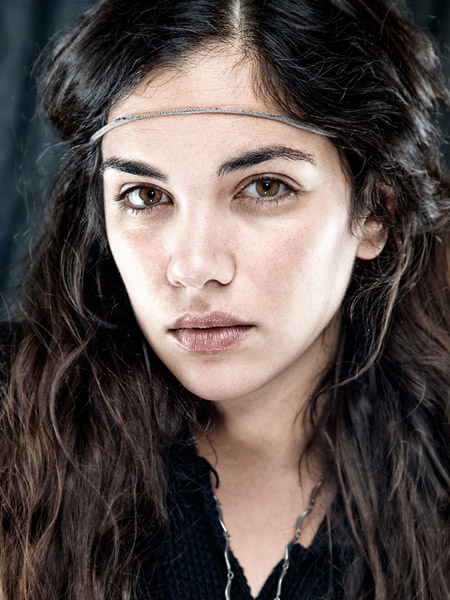
\includegraphics[width=1.5cm]{amato}}%
                    \hfill 
                   \medskip%
                }%
      }%
\end{texexample}

\begin{texexample}{}{}
    \fbox{%
          \vtop{\medskip
                    \hfill
                      \hbox{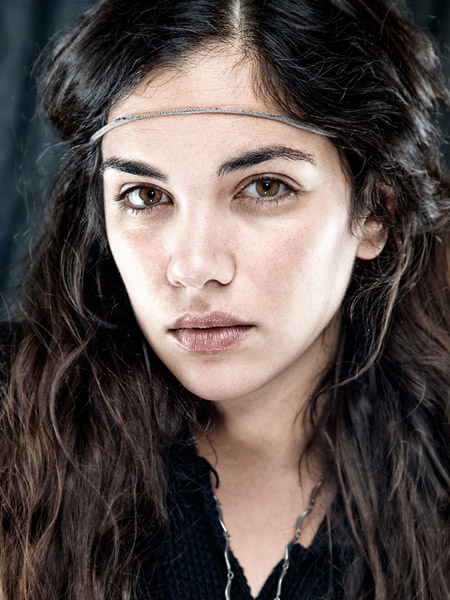
\includegraphics[width=1.5cm]{amato}}%
                      \hbox{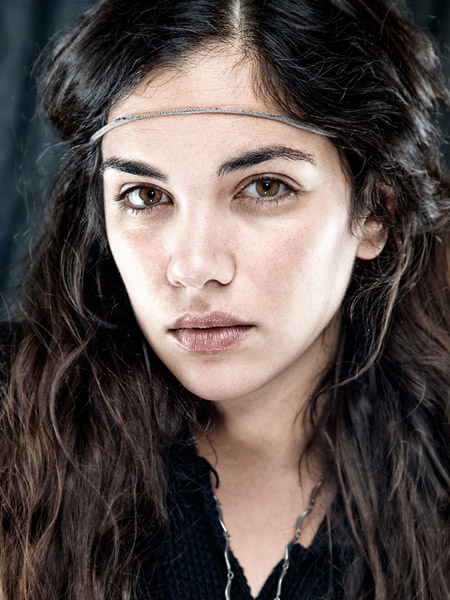
\includegraphics[width=1.5cm]{amato}}%
                      \hbox{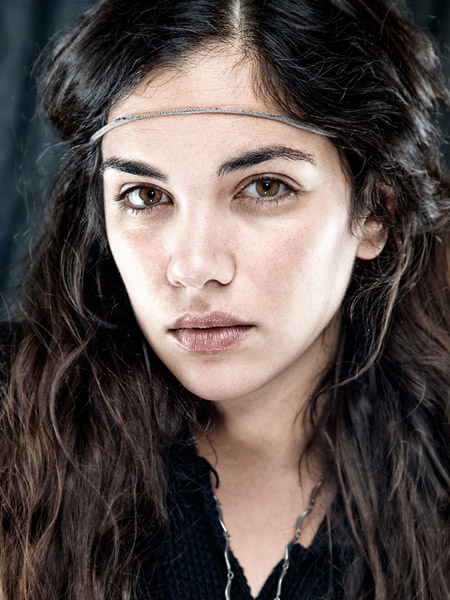
\includegraphics[width=1.5cm]{amato}}%    
                    \hfill 
                   \medskip%
                }%
      }%
\end{texexample}

Study the example a bit more carefully, as we have said earlier on that \cs{hbox}'es are stacked vertically, the reason why in the above example they are next to each other is that they are in an
\cs{fbox} which in turn is an \cs{hbox}  that can draw  frame around the box and is defined in the
\latex2e kernel.

So if we had only three images in hboxes we will get:

\begin{texexample}{}{}
\leavevmode
\parindent30pt
\hbox{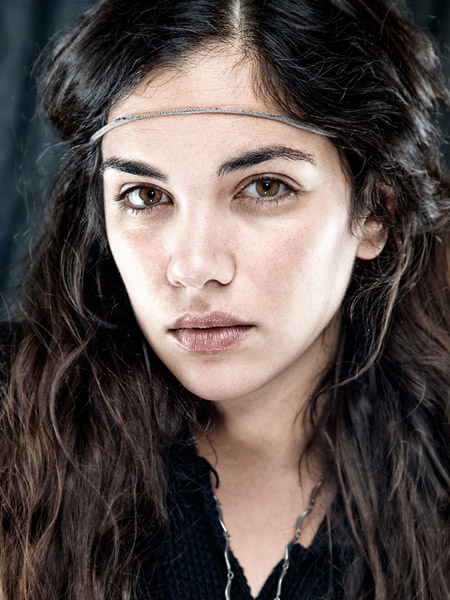
\includegraphics[width=1.5cm]{amato}}%
\hbox{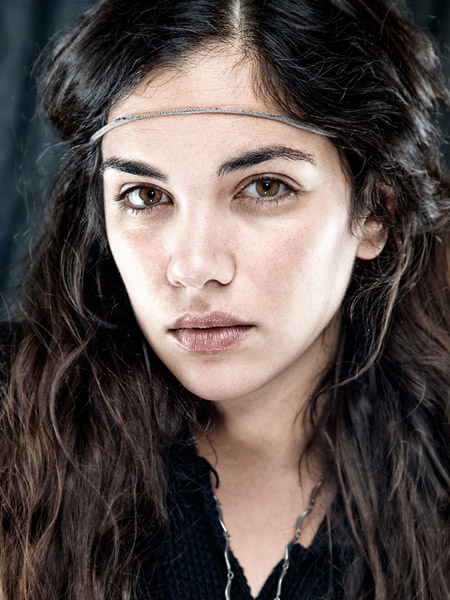
\includegraphics[width=1.5cm]{amato}}%
\hbox{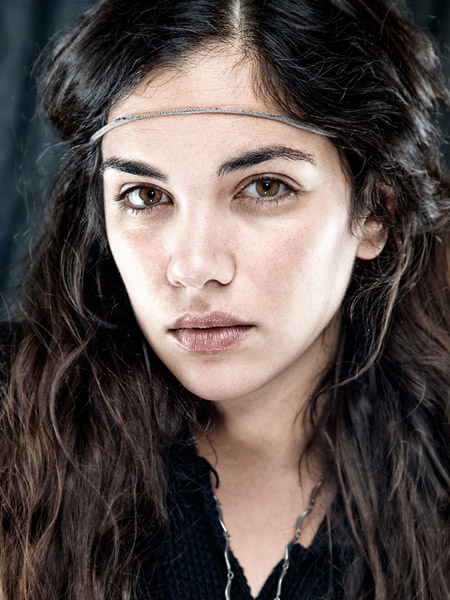
\includegraphics[width=1.5cm]{amato}}%
\end{texexample}

\begin{macro}{\kern}
If we wanted to add a bit of space between the horizontal images, we could use \cs{kern}
Kern again. This is from the book TeX for The Impatient page 157. You can use kern in math mode, but you cannot use the \texttt{mu} units. If you want to use \texttt{mu} units use \cs{mkern} instead.
\end{macro}

\begin{texexample}{}{}
   \fboxsep=0pt
   \fbox{%
          \vtop{\medskip
                    \hfill
                      \hbox{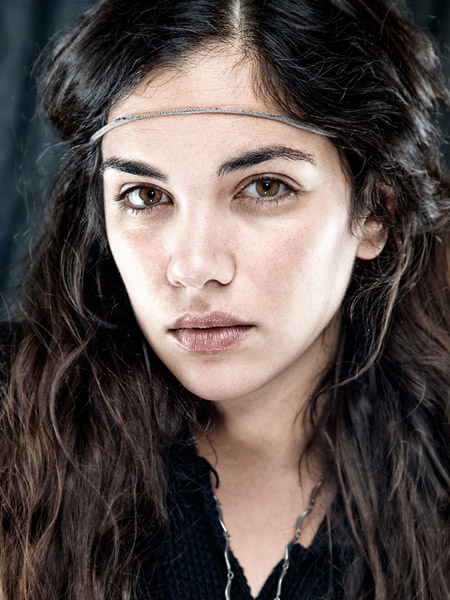
\includegraphics[width=1.5cm]{amato}}\kern10pt
                      \hbox{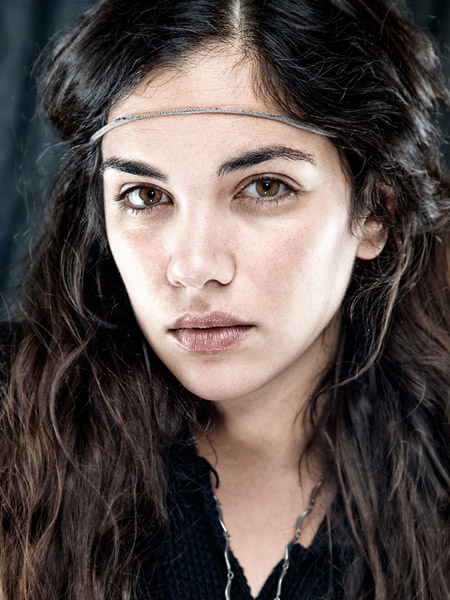
\includegraphics[width=1.5cm]{amato}}\kern10pt
                      \hbox{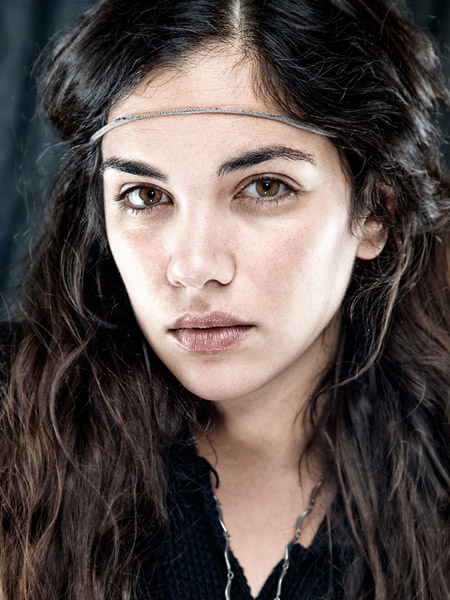
\includegraphics[width=1.5cm]{amato}}%    
                    \hfill 
                   \medskip%
                }%
   }%
\end{texexample}

\begin{texexample}{}{}
   \HHUGE
   \fboxsep=0pt
   \fbox{%
          \vtop{\medskip
                    \hfill
                       \hbox{ H\kern10pt i\kern10pt j}%    
                       \hbox{ A\kern10pt C\kern10pt j}%
                    \hfill 
                   \medskip%
                }%
   }%
\end{texexample}

This example shows how letters are typeset and you can see that they are aligned at the baseline. They are no different than the eimage example that we have shown earlier, except we don't need the boxes.

\medskip

\vbox{
\noindent\rule{\linewidth}{0.4pt}
\begin{minipage}{4.9cm}
\begin{teX}
\centerline{$\Downarrow$}\kern 3pt%
\centerline{$\Longrightarrow$\kern 6pt% horizontal kern
  \textit{A note about kern}\kern 6pt
    $\Longleftarrow$}
\kern 3pt
\centerline{$\Uparrow$}  
\end{teX}
\end{minipage}
\hspace{0.3cm}
\begin{minipage}{4.5cm}
\centerline{$\Downarrow$}\kern 3pt%
\centerline{$\Longrightarrow$\kern 6pt% horizontal kern
  \textit{A note about kern}\kern 6pt
    $\Longleftarrow$}
\kern 3pt
\centerline{$\Uparrow$}
\end{minipage}

\medskip
\noindent\rule{\linewidth}{0.4pt}
}
\medskip

To make a point again, |\vbox| lines boxes at their bottom while, |\vtop| lines them at their top.

\medskip

\vbox{
\noindent\rule{\linewidth}{0.4pt}
\begin{minipage}{4.9cm}
\begin{teX}
 \hbox{\hsize=2cm \raggedright
\vbox to 0.5in{\hrule This box is .5in deep. \vfil\hrule}
\qquad
\vbox to 0.75in{\hrule This box is .75in deep. \vfil\hrule}
\qquad
\end{teX}
\end{minipage}
\hspace{0.3cm}
\begin{minipage}{4.5cm}
\hbox{\hsize=2cm \raggedright
\vbox to 0.5in{\hrule This box is .5in deep. \vfil\hrule}
\qquad
\vbox to 0.75in{\hrule This box is .75in deep. \vfil\hrule}
\qquad}
\end{minipage}

\medskip
\noindent\rule{\linewidth}{0.4pt}
}

\medskip


Trying the same with vtop

\medskip

\vbox{
\noindent\rule{\linewidth}{0.4pt}
\begin{minipage}{4.9cm}
\begin{teX}
 \hbox{\hsize=2cm \raggedright
\vbox to 0.5in{\hrule This box is .5in deep. \vfil\hrule}
\qquad
\vbox to 0.75in{\hrule This box is .75in deep. \vfil\hrule}
\qquad
\end{teX}
\end{minipage}
\hspace{0.3cm}
\begin{minipage}{4.5cm}
\hbox{\hsize=2cm \raggedright
\vtop to 0.5in{\hrule \smallskip This box is .5in deep. \vfil\hrule}
\qquad
\vtop to 0.75in{\hrule \smallskip This box is .75in deep. \vfil\hrule}
\qquad}

\hbox{\hsize=2cm \raggedright
\vbox to 0.5in{\hrule \smallskip This box is .5in deep. \vfil\hrule}
\qquad
\vbox to 0.75in{\hrule \smallskip This box is .75in deep. \vfil\hrule}
\qquad}
\end{minipage}

\medskip
\noindent\rule{\linewidth}{0.4pt}
}

\medskip

There are some other special macros defined by Plain TeX that we will only touch briefly here. One of them is \cs{underbar}{\index{Plain!\textbackslash underbar}.
The macro puts its argument into an hbox and underlines it.

\medskip

\vbox{
\noindent\rule{\linewidth}{0.4pt}
\begin{minipage}{4.9cm}
\begin{teX}
 \underbar{1,000,788.22}
\end{teX}
\end{minipage}
\hspace{0.4cm}
\begin{minipage}{4.0cm}
\medskip
\hfill\hfill{}\hspace*{1em}a1,000,700.22 \hfill

\smallskip

\hfill\underbar{1,000,788.22}\hfill
\end{minipage}

\medskip
\noindent\rule{\linewidth}{0.4pt}
}

\medskip


The \cs{everyvbox} command inserts a series of tokens at the beginning of every |\vbox|.


\medskip

\vbox{
\noindent\rule{\linewidth}{0.4pt}
\begin{minipage}{4.9cm}
\begin{teX}
 \everyvbox{$\bullet$}...
\end{teX}
\end{minipage}
\hspace{0.4cm}
\begin{minipage}{4.0cm}
\begingroup% Without this group, there are tons of problems!
   \everyvbox{$\bullet$}
   \global\setbox1=\vbox{This is a paragraph without an initial indent. It is   \the\hsize\ long lines.}
   \global\setbox2=\vtop{\copy1}
\endgroup
 \hbox{\box1} 

 \hbox{\box2}
\end{minipage}

\medskip
\noindent\rule{\linewidth}{0.4pt}
}

\medskip
Knuth in the TexBook Chapter 24, has some short description of the every commands. The `everyhbox` inserts a token list just before as its name implies a horizontal box.

Here is a short example. We define a `oneLineBox`, which is simply an hbox with some text and we add spread to spread the line. Using |\everybox| we add the letter \textbf{a} in each horizontal box. 


\tex considers the box overfull if the excess width of the box is larger than \cs{hfuzz} or \cs{hbadness} is less than 100. If I change  the badness to hbadness, I get 1000.

\medskip

\vbox{
\noindent\rule{\linewidth}{0.4pt}
\begin{minipage}{10.0cm}
\begin{teX}
 \begingroup
     \everyhbox{a}
     \def\oneLineBox#1#2%
     {%
          \hfuzz=0pt
          \overfullrule=0.25pt
          \setbox0=\hbox spread#2{#1}%
          \setbox1=\hbox{\the\badness}% 
          \setbox2=\hbox to 4.5cm{\box0\hfil\box1}%
          \box2
     }
     \oneLineBox{Badness of line }{-1em}
     \oneLineBox{Badness of line }{-0.54em}
     \oneLineBox{Badness of line }{-0.4em}
     \oneLineBox{Badness of line }{0em}
     \oneLineBox{Badness of line }{1em}
     \oneLineBox{Badness of line }{2em}
     \oneLineBox{Badness of line }{3em}
 \endgroup
\end{teX}
\end{minipage}


\begin{minipage}{10.0cm}
\begingroup
     \everyhbox{a}
     \def\oneLineBox#1#2%
     {%
          \hfuzz=0pt
          \overfullrule=0.25pt
          \setbox0=\hbox spread#2{#1}%
          \setbox1=\hbox{\the\badness}% 
          \setbox2=\hbox to 4.5cm{\box0\hfil\box1}%
          \box2
     }
     \oneLineBox{Badness of line }{-1em}
     \oneLineBox{Badness of line }{-0.54em}
     \oneLineBox{Badness of line }{-0.4em}
     \oneLineBox{Badness of line }{0em}
     \oneLineBox{Badness of line }{1em}
     \oneLineBox{Badness of line }{2em}
     \oneLineBox{Badness of line }{3em}
 \endgroup
\end{minipage}

\medskip
\noindent\rule{\linewidth}{0.4pt}
}

\medskip



















\section{More features of horizontal boxes}

Characters in the Latin alphabet have different shapes, and in most typefaces,
different widths. The letters \texttt{d f h k l t} have ascenders, making them
higher than the vowels \texttt{a e o u}, while the letters \texttt{f g j p q y} have descenders,
giving them added depth below the vowels. Similarly, an \texttt{m} is wider than
an \texttt{i}. 

When \tex makes a normal horizontal box, the box width is the sum
of the widths of the characters, and the fixed parts of any glue, contained
in it. Shrink and stretch components of glue are discarded for the width
calculation. The box also has both a height above the baseline, the invisible
line on which the characters rest, and a depth below the baseline. The
depth is zero if there are no objects with descenders. The height and depth
are chosen from the largest vertical extents of the contained objects.

If you look carefully at typeset material, you will observe that, in most
typefaces, parentheses, brackets, and braces have both descenders and ascenders,
and the typeface designer usually makes their extents the maximum
among all of the characters in the design. This sample text shows
document: ( h g ) [ k j ] { l p }.

You can force TEX to choose a larger height and depth than normal when
you write a command for a horizontal box by ensuring that it has suitable
contents, such as an invisible vertical rule of zero width. The command

\verb+\hbox to 50pt {\vrule height 20pt depth 10pt width 0pt \it stuff}+

produces a box whose (invisible) outline looks like this: 

\hbox to 50pt {\vrule height 20pt depth 10pt width 0pt \it Great}

\noindent\fbox{\vrule height 20pt depth 10pt width 0pt \it Great}




The
three extents of the vertical rule can appear in any order, and any convenient
units.

\section{LaTeX Boxes}
In order to see the otherwise-invisible box edges in that example, we
used the \latex  built-in command \cs{fbox} to create a frame, and we eliminated
the default margin inside the frame by setting \cs{fboxsep = 0pt}. Plain TEX
does not have the \cs{fbox} command, but The TEXbook shows how to make
something like it on pp. 223 and 321.

One particular zero-width vertical rule is convenient for ensuring that
separate boxes all get the same height and depth. It has the height and
depth of parentheses in the normal prose font, and is given the macro name
\doccmd{strut}. Its definition in the plain.tex file of macro definitions is roughly
equivalent to this:

\begin{comment}
\begin{figure}[tbp]%
   \includegraphics[width=\linewidth]{./graphics/ascender}
   \caption{Boxes in \protect\TeX}
   \label{fig:ascender}
\end{figure}
\end{comment}

 \def \strut {\vrule height 8.5pt depth 3.5pt width 0pt}
\begin{teX}
  \def \strut {\vrule height 8.5pt depth 3.5pt width 0pt}
\end{teX}

Compare these two experiments with outlined boxes, first without struts,
and then with struts:




Notice the different vertical extents of the boxes in the first case, and how
they have identical extents in the second case.

\section{Horizontal alignment of boxes in TEX}

When horizontal boxes are set together, they are treated as separate words,
and therefore spaced accordingly. The input

\verb+ \fbox{one} \fbox{two} \fbox{three}\fbox{four}+  

produces  \fbox{one} \fbox{two} \fbox{three}\fbox{four}. As the example shows, we can put spaces
between them, or run them together so that they fit tightly.


\section{Vertical boxes in TEX}


\begin{minipage}{2.0in}
\begin{verbatim}
\noindent
\fbox{%
  \it
  \hbox to 80pt{%
     \parindent = 0pt
     \vbox to 30pt {%
         left text
         \vfil
         more left text%
     }%
  }%
}%
\end{verbatim}
\end{minipage}


%\noindent
\fbox{%
  \it
  \hbox to 80pt{%
     \parindent = 0pt
     \vbox to 30pt {%
         left text
         \vfil
         more left text%
     }%
  }%
}%

Firstly we use a noindent to ensure that the box is not indented. If you comment the\cs{fbox} out, you can see that the right amount of space has been left in the paragraph above.

\mbox{}
 
\noindent
\fbox{%
\it
\hbox to 80pt{%
\parindent = 0pt
\hsize = 80pt
\vbox to 30pt {\hfill right text
\vfil
\hfill more right text}
}%
}%



\noindent
\fbox{%
\it
\hbox to 80pt{%
\parindent = 0pt
\hsize = 80pt
\vbox to 30pt {\hfil center text
\vfil
 more center text \hfil}
}%
}%

We can aslo center the text for both lines, by modifying the code slightly.
\begin{teX}
\noindent
\fbox{%
\it \hbox to 80pt{
   \parindent = 0pt
   \hsize = 80pt
   \vbox to 30pt {
   center text \hfill
    \vfil
    \hfil more center text}
   }%
}%
\end{teX}


\noindent
\fbox{%
\it
\hbox to 80pt{%
\parindent = 0pt
\hsize = 80pt
\vbox to 30pt {\hfil center text
\vfil
\hfil more center text}
}%
}%



\chapter{Boxes with \protect\LaTeXe}

A  box of specified width is provided in \latex with the command:

\cs{makebox}\oarg{width}\oarg{position}\marg{contents}. 

The source2e manual states. If the width is missing, then position is also missing and obj  is put in an \cs{hbox} of its natural width. This is true as far as the looks are concerned, but not the behaviour, as you can see
from the following example is not an unqualified hbox it is an hbox preceded by leavevmode.\footnote{\url{http://tex.stackexchange.com/questions/105585/latex2e-makebox-hbox}} This is of course good practice and brings consistency to the LaTeX kernel. I would recommend that you follow such practices in your own code. 

\begin{texexample}{}{}
\newbox\temp
\savebox\temp{test}
LaTeX

\makebox{test} \mbox{test}

TeX

\hbox{test} \hbox{test}

\indent\hbox{test} \hbox{test}

LaTeX with \cs{leavemode}

\makeatletter
\leavevmode\hbox to \wd\temp{test} \indent\hbox to \wd\temp{test}
\makeatother
\end{texexample}



\latex's analog of a\cs{hbox} is called \cs{mbox}. They are 
much the same thing, but \cs{mbox} is defined to be more widely usable. We have already used \latex's framed companion to \cs{mbox}, \cs{fbox}.

A horizontal box of specified width is provided in \latex with the command
\doccmd{makebox[width][position]\{contents\}}. Bracketed command arguments
in \latex are always optional. 

Here, the width is a TEX dimension,
and defaults to the natural width of the contents if not given. The position
is one of the letters \textbf{l} (flush left) or \textbf{r} (flush right); if it is omitted, the text
is centered in the box. If the specified width is smaller than needed, the
contents protrude from the box, and may overlap surrounding material. If
the specified width is zero, then we have equivalents of the TEX \cs{rlap} and
\cs{llap} commands.


Here are several examples of these three LATEX box commands:

{\obeylines
\mbox{stuff}

\fbox{stuff} 

|\makebox{stuff}|

|\makebox[40pt][l]{stuff}|

|\makebox[40pt][r]{stuff}|

|\makebox[0pt]{stuff}|

|\makebox[0pt][l]{stuff}|

|\makebox[0pt][r]{stuff}|
}


The \cs{makebox} command has a framed companion, \cs{framebox}, with identical
arguments. Like \cs{fbox}, \cs{framebox} creates a margin of width \cs{fboxsep}
between the outline and the contents, but we continue with a zero value for
that separation:



\framebox{stuff} 

\framebox[40pt][l]{stuff} 

\framebox[40pt][r]{stuff}

\framebox[0pt]{stuff} 

\framebox[0pt][l]{stuff} 

\framebox[0pt][r]{stuff}

The last three examples show that the frame shrinks to a vertical bar when
the box width is zero.

To help in positioning boxes within other objects, \latex provides the command
\cs{raisebox} to raise and lower boxes:

\begin{teX}
\raisebox{raiselength}[height][depth]{contents}
\end{teX}

A negative first argument lowers the box. Here are some examples:


A \raisebox{10pt}{\fbox{upper}} A
upper
A \raisebox{10pt}{\
fbox{lower}} A
lower
A \fbox{\raisebox{10pt}[25pt]{\fbox{upper}}} A
upper
A \fbox{\raisebox{10pt}[
25pt]{\fbox{lower}}} A
lower
A \fbox{\raisebox{10pt}[25pt][15pt]{\fbox{upper}}} A
upper
A \fbox{\raisebox{10pt}[
25pt][15pt]{\fbox{lower}}} A
lower

\section{Paragraph Boxes}

For longer strings of text, \latex provides the paragraph box \cs{parbox}, which is
defined like this: 

\medskip
\cs{parbox}\oarg{position}\oarg{height}\oarg{innerpos}\marg{width}\marg{contents} 
\medskip

The optional position
is a letter b for alignment of the bottomline with the current baseline,
or t for alignment of the top line with the surrounding baseline. Without

The box can be used as if it were a letter or a word, so we can put it in
the middle of a sentence. The input

This is text \parbox{30pt}{\it and this is boxed text} and
this is more text.

This is text \fbox{\parbox{30pt}{\it and this is boxed text}}
and this is more text.
produces


Flush-right typesetting generally looks bad in narrow columns, so we
can insert a \cs{raggedright} command inside the last argument of the paragraph
box to get output like this:

\begin{texexample}{}{}

\parbox[b][120pt][t]{100pt}{\lorem}\hspace{1cm}\parbox[b][120pt][t]{100pt}{Only some short line of text here.}



\parbox[b][100pt][t]{100pt}{\lorem}\hspace{1cm}\parbox[b][100pt][c]{100pt}{Only some short line of text here.}

\end{texexample}


\section*{The minipage environment}

Another kind of paragraph box can be obtained in a more general, and
more powerful, way with the minipage environment:

\begin{teX}
\begin{minipage}[position]{width}
   contents
\end{minipage}
\end{teX}


The positioning works just like that for \verb+ \parbox+, with alignment letters b
and t, and if they are omitted, a default of vertical centering.
In particular, verbatim text produced with the verb command is illegal
in macro arguments, so it cannot be used with \cs{fbox}, \cs{framebox}, \cs{makebox},
\cs{mbox}, or\cs{ parbox}, but it can be used inside a minipage. The input


\begin{texexample}{}{}
\begin{minipage}{170pt}
This is inline verbatim \verb=\verb|\%{}|=, and this
is a verbatim display:

\begin{verbatim}
#include <stdio.h>
#include <stdlib.h>
int main(void)
{
  printf("Hello, world\n");
  exit (EXIT_SUCCESS);
}
\end{verbatim}
\end{minipage}

\end{texexample}


A minipage can go everywhere and can hold virtually any content.





\section{Scaling and resizing boxes}

The command \cs{resizebox}\marg{width}\marg{height}\marg{object} can be used with tabular to specify the height and width of a table. The following example shows how to resize a table to 8cm width while maintaining the original width/height ratio.

\begin{teX}
\resizebox{8cm}{!} {
  \begin{tabular}...
  \end{tabular}
}
\end{teX}

Alternatively you can use \cs{scalebox}{ratio}{object} in the same way but with ratios rather than fixed sizes:

\begin{teX}
\scalebox{0.7}{
  \begin{tabular}...
  \end{tabular}
}
\end{teX}

Both |\resizebox| and |\scalebox| require the \docpkg{graphicx} package.
To tweak the space between columns (LaTeX will by default chose very tight columns), one can alter the column separation: |\setlength{\tabcolsep}{5pt}|. The default value is |6pt|.

The scalebox is great if you want to magnify a letter so that you can observe the design closer.

\bigskip
\noindent\begin{tabular}{|c|c|c|c|c|c|}\hline
Kp-Fonts & Kp-\textit{light} & CM & Palatino & Utopia & Times\\\hline\hline
\scalebox{2}{ag713} &
\scalebox{2}{\fontfamily{jkpl}\selectfont 7} &
\scalebox{2}{\fontfamily{lmr}\selectfont 713}  &
\scalebox{2}{\fontfamily{ppl}\selectfont 713}  &
\scalebox{2}{\fontfamily{put}\selectfont 7} &
\scalebox{2}{\fontfamily{ptm}\selectfont \oldstylenums{7}} \\\hline
\end{tabular}


\begin{teX}
\hspace{-6mm}\begin{tabular}{|c|c|c|c|c|c|}\hline
Kp-Fonts & Kp-\textit{light} & CM & Palatino & Utopia & Times\\
\hline\hline
  \scalebox{10}{a} &
  \scalebox{10}{\fontfamily{jkpl}\selectfont a} &
  \scalebox{10}{\fontfamily{lmr}\selectfont a}  &
  \scalebox{10}{\fontfamily{ppl}\selectfont 7}  &
  \scalebox{9.2}{\rule{0pt}{1.25ex}\fontfamily{put}\selectfont a} &
  \scalebox{10}{\fontfamily{ptm}\selectfont a}\\\hline
\end{tabular}
\end{teX}
\bigskip


















